\ifdefined\COMPLETE
\else
    \input{./preambule-sacha-utf8.ltx}
    \begin{document}
\fi


\vspace*{-.5cm}

\setcounter{section}{0} 

\part{Fonctions numériques de la variable réelle}

\section{Généralités}

\subsection{Fonctions}

\begin{tabular}{lll}
Soit & $f:$ & $ \R \rightarrow \R$ \\
& & $x\mapsto \underbrace{f(x)}_{\textrm{image de} x}$ \\
\end{tabular}

$f$ est une fonction numérique de la variable réelle si et seulement si :

\textbf{Tout élément de $\mathbf{\R}$ a au plus une image dans $\mathbf{\R}$.} \\

\textbf{Remarques}

\begin{itemize}


\item[*]Vocabulaire : "Au plus une" veut dire, soit une, soit aucune. \\ 

\item[*] $f$ est une fonction et $f(x)$ un nombre réel.
\end{itemize}
\subsection{Ensemble de définition d'une fonction}

\begin{tabular}{lll}

Soit & $f:$& $ \R \rightarrow \R$ \\
& & $x\mapsto f(x)$ \\
\end{tabular}

\vspace*{.3cm}

\textbf{L'ensemble de définition de f, noté $ \mathbf{D_f} $, est l'ensemble de élément de $\mathbf{\R}$\\qui ont une image dans $\mathbf{\R}$}. \\

\vspace*{.3cm}

\begin{minipage}{5cm}
\begin{tikzpicture}[scale=.8]

\tkzDefPoint [label=left:$a$](0,1.5){a}
\tkzDrawPoint[size=10,color=black](a)
\tkzDefPoint [label=left:$b$](0,1){b}
\tkzDrawPoint[size=10,color=black](b)
\tkzDefPoint [label=left:$c$](0,.5){c}
\tkzDrawPoint[size=10,color=black](c)
\tkzDefPoint [label=left:$d$](0,0){d}
\tkzDrawPoint[size=10,color=black](d)
\tkzDefPoint [label=right:$\Delta$](3,1.5){de}
\tkzDrawPoint[size=10,color=black](de)
\tkzDefPoint [label=right:$\bigstar$](3,1){st}
\tkzDrawPoint[size=10,color=black](st)
\tkzDefPoint [label=right:$\bigcirc$](3,.5){nada}
\tkzDrawPoint[size=10,color=black](nada)



\node [draw,ellipse,minimum height=3cm,minimum width=1.5cm, fit={(a) (b) (c) (d) }] {};
\node [draw,ellipse,minimum height=3cm,minimum width=1cm,fit={(de) (st) (nada) }] {};

\draw  [bend left=20,-latex](a) to (de) ; 
\draw  [bend right=20,-latex](b) to (de) ; 
\draw  [bend right=20,-latex](c) to (st) ; 
\end{tikzpicture}
\end{minipage}
\begin{minipage}{3cm}

$f(a) = \Delta$

$f(b) = \Delta$

$f(c) = \bigstar $ \\

$ D_f = \lb a, b, c \rb $

$D_f = E \setminus\lb d \rb $

\end{minipage}\\


\subsubsection{Exercice \no 1}

\begin{tabular}{llll}
Soit & $f:$& $ \R \rightarrow \R$ & \\
& & $x\mapsto f(x)$ & $=\dfrac{x-1}{x+1}$ \\
\end{tabular}\\

Il ne faut pas que $x+1=0$, donc que $x=-1$.

$D_f = \R \setminus \lb -1 \rb = \left]-\infty,-1\right[\cup\left]-1, +\infty\right[$

\subsubsection{Exercice \no 2}

\begin{tabular}{llll}

Soit & $f:$& $ \R \rightarrow \R$ & \\
& & $x\mapsto f(x)$ & $=\sqrt{x+2}$ \\
\end{tabular}\\

Il faut que $x+2 \geqslant 0$, donc que $x \geqslant -2 $

$D_f = \left[-2, +\infty\right[ $

\newpage

\subsubsection{Exercice \no 3}

\begin{tabular}{llll}

Soit & $f:$& $ \R \rightarrow \R$ & \\
& & $x\mapsto f(x)$ & $=\dfrac{x^2 + 4}{x^2 - 4}$ \\
\end{tabular}\\

Il ne faut pas que $x^2 - 4 = 0$, donc que $\left(x+2\right)\left(x-2\right) = 0 $

\begin{tabular}{lll}
$x+2=0$ & ou & $x-2 = 0 $ \\
$x = -2 $ & ou & $x=2$ \\
\end{tabular}

$ D_f = \R \setminus\lb -2,2\rb = \left]-\infty, -2\right[\cup \left]-2,2\right[\cup\left]2, +\infty\right[ $

\subsubsection{Exercice \no 4}

\begin{tabular}{llll}

Soit & $f:$& $ \R \rightarrow \R$ & \\
& & $x\mapsto f(x)$ & $=\dfrac{x^2 - 4}{x^2 + 4}$ \\
\end{tabular}\\

Il ne faut pas que $x^2 + 4 = 0$, donc que $x^2 = -4 $. \\

Or, $x^2 = -4$ n'a pas de solution dans $\R$. \\

D'où $D_f = \R = \left]-\infty \; ; \; +\infty\right[$.

\subsubsection{Exercice \no 5}

\begin{tabular}{llll}

Soit & $f:$& $ \R \rightarrow \R$ & \\
& & $x\mapsto f(x)$ & $=\sqrt{x^2 - 1}$ \\
\end{tabular}

Il faut que $x^2 - 1 \geqslant 0 $.

\begin{tikzpicture}
\tkzTabInit[lgt=3,espcl=2]
{ $x$  /1,
$x^2+1$ /1}
{$ - \infty $ , $-1 $ , $1$ , $ + \infty $}
\tkzTabLine{ , + , z , - , z , + }
\end{tikzpicture}

$D_f = \left]-\infty,-1\right]\cup\left[1,+\infty\right[ $

\subsubsection{Exercice \no 6}

\begin{tabular}{llll}

Soit & $f:$& $ \R \rightarrow \R$ & \\
& & $x\mapsto f(x)$ & $=\sqrt{x^2 + 1}$ \\
\end{tabular}

Il faut que $x^2+1 \geqslant 0$, donc $x^2 \geqslant -4$

Ceci est toujours vrai, donc $D_f = \R$.

\newpage

\subsection{Exercice d'application}

Étudier les fonctions $f$ et $g$ suivantes : \\

\begin{tabular}{ll}
\begin{tabular}{llllll}
Soit $f$ : & $\R$ & $\longrightarrow$ & $\R$ & & \\
& $x$ & $\longmapsto$ & $f\left(x\right)$ & $=$ & $\sqrt{\dfrac{-x^2 + 3x + 10}{x^2 + 4x -21}}$ \\
\end{tabular}

\vspace*{.3cm}

&

\begin{tabular}{llllll}
Soit $g$ : & $\R$ & $\longrightarrow$ & $\R$ & & \\
& $x$ & $\longmapsto$ & $g\left(x\right)$ & $=$ & $\dfrac{\sqrt{-x^2 + 3x + 10}}{\sqrt{x^2 + 4x -21}}$ \\
\end{tabular}

\vspace*{.3cm} \\

Il faut que $\dfrac{-x^2 + 3x + 10}{x^2 + 4x -21} \geqslant 0$. \vspace*{.3cm} & Il faut que $\begin{cases}
-x^2 + 3x + 10 \geqslant 0 \\
x^2 + 4x -21 > 0 \\
\end{cases}$ \\

Il ne faut pas que $x^2 + 4x - 21 = 0$. \vspace*{.3cm} \\

\vspace*{.3cm} On étudie le trinôme $-x^2 + 3x + 10$ & On étudie le trinôme $-x^2 + 3x + 10$ \\

\vspace*{.3cm} $-x^2 + 3x + 10 = 0$ pour $x = -2$ ou $x=5$. & $-x^2 + 3x + 10 = 0$ pour $x = -2$ ou $x=5$.\\

\vspace*{.3cm} On étudie le trinôme $x^2 + 4x -21$ & On étudie le trinôme $x^2 + 4x -21$ \\

\vspace*{.3cm} $x^2 + 4x -21 = 0$ pour $x = -7$ ou $x=3$. & $x^2 + 4x -21 = 0$ pour $x = -7$ ou $x=3$. \\ 

On peut dresser le tableau de signes suivant : & On peut dresser les tableaux de signes suivants : \\

\begin{tikzpicture}
\tkzTabInit[lgt=2.5,espcl=1]
{ $x$  /1,
$-x^2+3x + 10$ /1,
$x^2+4x - 21$ /1,
$\dfrac{-x^2 + 3x + 10}{x^2 + 4x -21}$ /1}
{$ - \infty $ , $-7 $ , $-2$, $3$, $5$ , $ + \infty $}
\tkzTabLine{ , - , t , - , z , + , t , + , z , - }
\tkzTabLine{ , + , z , - , t , - , z , + , t , + }
\tkzTabLine{ , - , d , + , z , - , d , + , z , - }
\end{tikzpicture}

&

\vspace*{-4.2cm}

\begin{tikzpicture}
\tkzTabInit[lgt=2.5,espcl=1.5]
{ $x$  /1,
$-x^2+3x + 10$ /1}
{$ - \infty $ , $-2 $ , $5$ , $ + \infty $}
\tkzTabLine{ , - , z , + , z , - }
\end{tikzpicture}

\\

& 

\vspace*{-.1cm}

\begin{tikzpicture}
\tkzTabInit[lgt=2.5,espcl=1.5]
{ $x$  /1,
$x^2+4x + -21$ /1}
{$ - \infty $ , $-7 $ , $3$ , $ + \infty $}
\tkzTabLine{ , + , z , - , z , + }
\end{tikzpicture}

\vspace*{2.3cm}

\\

On a donc $D_f = \left]-7 \; ; \; -2 \right]\cup \left]3 \; ; \; 5 \right]$ & On a $S_1 = \left[-2 \; ; \; 5\right]$ et $S_2 = \left]-\infty \; ; \; -7\right[ \cup \left] 3 \; ; \; +\infty\right[$. \\

& $D_g = S_1 \cap S_2 = \left]3 \; ; \; +\infty\right[$. \\
\end{tabular}

\vspace*{.5cm}

\textbf{Conclusion générale :}

Les fonctions $f$ et $g$ ne sont pas égales, car $D_f \neq D_g$. \\

Ici, on peut noter que $D_g \subset D_f$. 


\ifdefined\COMPLETE
\else
    \end{document}
\fi